\chapter{Relevante GSM-Abläufe} \label{hdl:grundlagen_ablufe}

Im Folgenden werden verschiedene Abläufe in \ac{GSM} anhand von Nachrichtenflussdiagrammen oder Wireshark-Mitschnitten aufgelistet.

\section{\acl{RR} Connection Establishment} \label{hdl:grundlagen_rr-conn-est}

Neben den \ac{BCCH} und \ac{CCCH} gibt es in \ac{GSM} noch die dedizierten logischen Kanäle, bei denen eine Verbindung zwischen je einem \ac{MS} und einem \ac{BTS} aufgebaut wird. Der interne Nachrichtenaustausch zwischen den Protokollschichten läuft über \acp{SAP}.

Um bidirektional über einen solchen Kanal kommunizieren zu können, ist der Aufbau einer \ac{LAPDm} und darauf aufbauend einer \ac{RR} Verbindung notwendig. Die Signalisierung, die zur Einrichtung und Auflösung einer \ac{RR}-Verbindung nötig ist, wird in \autoref{fig:rr-conn-est} dargestellt.

\begin{figure}[H]
  \begin{center}
    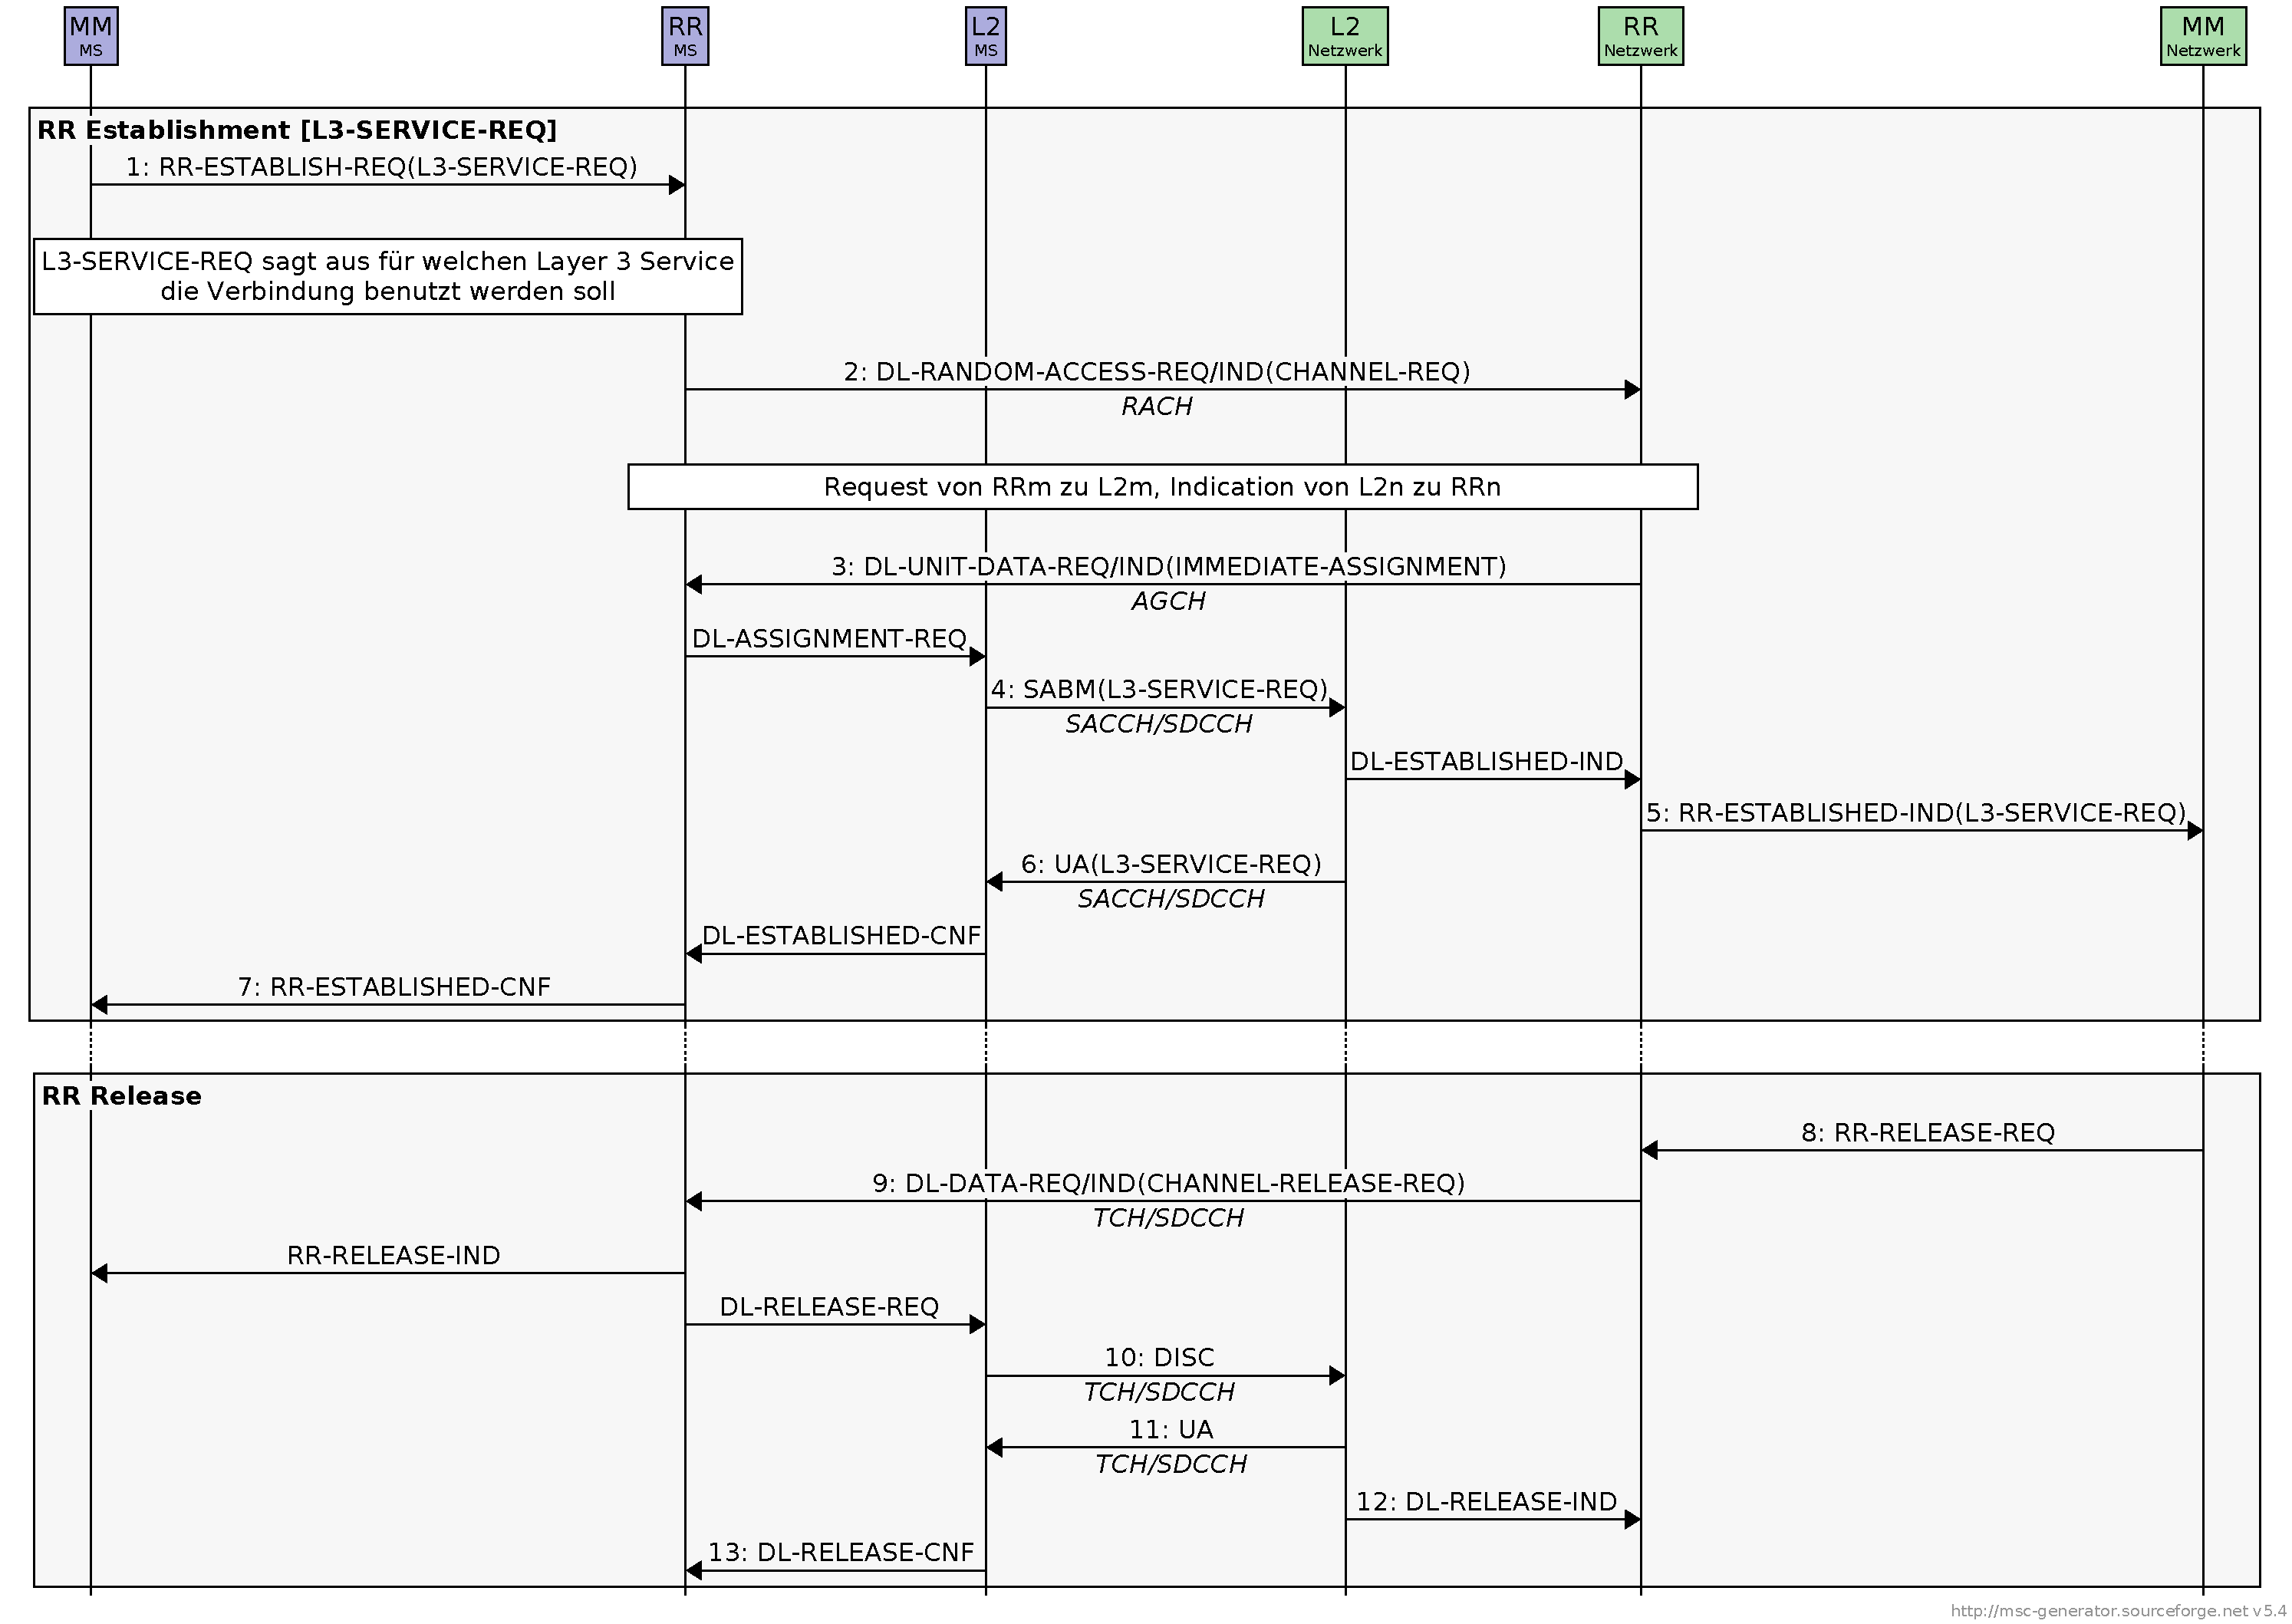
\includegraphics[width=1.00\textwidth]{figures/gsm_rr-chan-est-rel.pdf}
  \end{center}
  \caption[Nachrichtenfluss von RR-Verbindungsaufbaus und Release]{Nachrichtenfluss von \ac{RR}-Verbindungsaufbau und Release} \label{fig:rr-conn-est}
\end{figure}

\begin{description}
\item[1] Der Verbindungsaufbau wird durch ein \texttt{RR-ESTABLISH-REQ} Primitive vom $\ac{MM}_{MS}$ an das \ac{SAP} des $\ac{RR}_{MS}$ in Auftrag gegeben. Entweder initiativ vom \ac{MS}, oder als Reaktion einer eingehenden Paging Nachricht auf dem \ac{PCH}.
\item[2] $\ac{RR}_{MS}$ lässt daraufhin von der physikalischen Schicht auf dem \ac{RACH} eine \texttt{CHANNEL-REQUEST}-Nachricht an $\ac{RR}_{Netzwerk}$ schicken. Wir sehen in \autoref{fig:interface-physical-layer}, dass diese einen \ac{SAP} direkt für \ac{RR} zur Verfügung stellt, die Datensicherungsschicht \ac{LAPDm} wird dabei übergangen.
\item[3] $\ac{RR}_{Netzwerk}$ reserviert entsprechende Ressourcen auf einem der dedizierten Kanäle. Das ist bei Early und Late-Assignment ein \ac{SDCCH} und bei Very-Early-Assignment bereits der \ac{TCH}. Über den \ac{AGCH} werden $\ac{RR}_{MS}$ in einer \texttt{IMMEDIATE-ASSIGNMENT}-Nachricht anschließend Informationen zum reservierten Kanal mitgeteilt. Schicht 2 wird wieder übergangen.
\item[4] Nach Erhalt des Immediate-Assignments wechselt das \ac{MS} in den "`Dedicated Mode"' und empfängt nur noch Nachrichten auf dem zugewiesenen dedizierten Kanal. \ac{BCCH}, \ac{CCCH} werden ignoriert. Eine zuverlässige Verbindung (\autoref{hdl:einfuehrung-gsm_schnittstellen_protokolle-um_interface-layer2}) wird von $L2_{MS}$ über die \ac{LAPDm}-Nachricht \ac{SABM} im unacknowledged Mode initiiert \citepauthor[3.8.2]{3gpp:04.06}.
\item[5] \ac{SABM} trägt dabei den kompletten von $\ac{MM}_{MS}$ in Auftrag gegebenen Service Request (\texttt{L3-SERVICE-REQUEST}) mit sich, was "`piggybacking"' genannt wird. Nachdem $L2_{Netzwerk}$ über den \ac{SAP} mit einer \texttt{DL-ESTABLISHED-IND} $\ac{RR}_{Netzwerk}$ über die Einrichtung der zuverlässigen Verbindung informiert hat, schickt dieses den Service Request weiter an $\ac{MM}_{Netzwerk}$. 
\item[6] Mit der \ac{LAPDm}-Nachricht \ac{UA} wird $L2_{MS}$ angewiesen, nun in den Acknowledged Information Transfer Mode zu wechseln. Ab dann werden durchnummerierte \ac{I}-Frames geschickt und die Verbindung ist durch die Retransmission Prozeduren, \ac{ACK} und \ac{REJ}-Nachrichten von Schicht 2 vor Paketverlust geschützt.
\item[7] Durch entsprechende \ac{SAP} Confirm Primitives werden $\ac{RR}_{MS}$ und $\ac{MM}_{MS}$ über die aufgebaute zuverlässige Verbindung informiert. Schicht 3 kann nun über \ac{LAPDm} auf diese zugreifen und Daten übertragen. Im Anschluss kann die Signalisierung für Authentifizierung und Verschlüsselung ablaufen, wofür die zuverlässige Verbindung benötigt wird. \citepauthor[3.3]{3gpp:04.18} \citepauthor[Figure A.1 ff.]{3gpp:24.007}
\item[8] In der Abbildung initiiert $\ac{MM}_{Netzwerk}$ das Auflösen der Verbindung mit einem \texttt{RR-RELEASE-REQ}, was aber auch vom \ac{MS} ausgehen kann.
\item[9] Der \texttt{CHANNEL-RELEASE-REQUEST} wird an $\ac{RR}_{MS}$ weitergeleitet.
\item[10] $\ac{RR}_{MS}$ reagiert indem es $\ac{MM}_{MS}$ über die beendete Verbindung informiert und $L2_{MS}$ befiehlt, diese aufzulösen. $L2_{MS}$ kommt dem nach und informiert über \ac{LAPDm} \texttt{DISC} $L2_{Netzwerk}$ über den Wechsel in den Unacknowledged Information Transfer Mode, der mit einem \ac{UA} Frame bestätigt wird.
\item[11] Erhält $\ac{RR}_{MS}$ die Bestätigung über das Beenden der zuverlässigen Verbindung, wechselt das \ac{MS} vom "`Dedicated"' wieder in den "`Idle Mode"'. Es werden also wieder Nachrichten auf \ac{BCCH} und \ac{CCCH} empfangen und bearbeitet. \citepauthor[3.4.13]{3gpp:04.18} \citepauthor[Figure A.1 ff.]{3gpp:24.007}
\end{description} 

\section{Wireshark Mitschnitte}

Im Folgenden sind Mitschnitte des Nachrichtenverkehrs auf dem \ac{Um} aufgelistet. Mitschnitte \autoref{lst:real_bts_traffic_det_wireshark} und \autoref{lst:real_bts_traffic_short_wireshark} wurden von osmocomBB mit aktivem \ac{GSMTAP} Logging erstellt. Die Destination-\ac{IP}-Adresse ist deshalb immer das lokale Netzwerkinterface. \autoref{lst:mitm_attack_wireshark} zeigt den aufgezeichneten \ac{MitM}-Angriff auf dem virtuellen \ac{Um}. Dabei sind die \ac{MS} unter der \ac{IP}-Adresse 226.0.0.1 zu erreichen, der \ac{MitM} unter 226.0.0.1 und die \ac{BTS}. Da sowohl die Verbindung von \ac{MS} zu \ac{MitM}, als auch von \ac{MitM} zu \ac{BTS} aufgezeichnet wird, scheinen manche Nachrichten doppelt zu sein. In \autoref{lst:mitm_attack_wireshark} wurden die Details von interessanten Nachrichten aufgeklappt.

Der in Wireshark angewendete Filter für den detaillierten Nachrichtenverlauf mit \ac{LAPDm}"=Kontrollnachrichten ist: 
\begin{verbatim}
   !(gsmtap.chan_type == 137) 
&& !(gsmtap.chan_type == 136) 
&& !(gsm_a.dtap.msg_rr_type == 0x15) 
&& lapdm
\end{verbatim}
Für den detaillierten Nachrichtenverlauf mit \ac{LAPDm}-Kontrollnachrichten ist der Filter:
\begin{verbatim}
   !(lapdm.length_field == 0x01) 
&& !(gsmtap.chan_type == 137) 
&& !(gsmtap.chan_type == 136) 
&& !(gsm_a.dtap.msg_rr_type == 0x15) 
&& lapdm
\end{verbatim}

Kommentare in den Mitschnitten werden in blau angezeigt und sind nicht Teil der Nachrichten. Manipulierte Nachrichten in \autoref{lst:mitm_attack_wireshark} sind rot gekennzeichnet.\\

\begin{lstlisting}[caption={[Aufgezeichneter Nachrichtenverkehr mit E-plus BTS, kurz]Aufgezeichneter Nachrichtenverkehr mit E-plus \ac{BTS}, kurz (ohne \ac{LAPDm}-Kontrollnachrichten), generiert mit Filtern aus Wireshark-Mitschnitt}, label={lst:real_bts_traffic_short_wireshark}, boxpos=c, frame=single, language=bytetxt, numbers=none, basicstyle=\tiny\ttfamily, tabsize=1 ]
No.     Destination           Protocol 
    293 127.0.0.1             LAPDm    U P, func=SABM(DTAP) (MM) Location Updating Request 
    298 127.0.0.1             LAPDm    U F, func=UA(DTAP) (MM) Location Updating Request 
    299 127.0.0.1             LAPDm    I, N(R)=0, N(S)=0(DTAP) (MM) Identity Request 
    301 127.0.0.1             LAPDm    I, N(R)=1, N(S)=0(DTAP) (MM) Identity Response 
    303 127.0.0.1             LAPDm    I, N(R)=0, N(S)=1(DTAP) (MM) Identity Request 
    307 127.0.0.1             LAPDm    I, N(R)=2, N(S)=1(DTAP) (MM) Identity Response 
    309 127.0.0.1             LAPDm    I P, N(R)=1, N(S)=1(DTAP) (MM) Identity Request 
    313 127.0.0.1             LAPDm    I, N(R)=2, N(S)=2(DTAP) (MM) Authentication Request 
    323 127.0.0.1             LAPDm    I, N(R)=3, N(S)=2(DTAP) (MM) Authentication Response 
    329 127.0.0.1             LAPDm    I, N(R)=3, N(S)=3(DTAP) (RR) Ciphering Mode Command 
    331 127.0.0.1             LAPDm    I, N(R)=4, N(S)=3(DTAP) (RR) Ciphering Mode Complete 
    333 127.0.0.1             LAPDm    I, N(R)=4, N(S)=4(DTAP) (MM) Identity Request 
    335 127.0.0.1             LAPDm    I, N(R)=5, N(S)=4(DTAP) (MM) Identity Response 
    339 127.0.0.1             LAPDm    I, N(R)=5, N(S)=5(DTAP) (MM) Location Updating Accept 
    341 127.0.0.1             LAPDm    I, N(R)=6, N(S)=5(DTAP) (MM) TMSI Reallocation Complete 
    348 127.0.0.1             LAPDm    I, N(R)=5, N(S)=6 (Fragment)
    353 127.0.0.1             LAPDm    I P, N(R)=6, N(S)=6 (Fragment)
    355 127.0.0.1             LAPDm    I, N(R)=6, N(S)=7(DTAP) (MM) MM Information 
    357 127.0.0.1             LAPDm    I, N(R)=6, N(S)=0(DTAP) (RR) Channel Release 
   2987 127.0.0.1             LAPDm    U P, func=SABM(DTAP) (MM) CM Service Request 
   2992 127.0.0.1             LAPDm    U F, func=UA(DTAP) (MM) CM Service Request 
   2994 127.0.0.1             LAPDm    I, N(R)=0, N(S)=0(DTAP) (MM) Identity Request 
   2996 127.0.0.1             LAPDm    I, N(R)=1, N(S)=0(DTAP) (MM) Identity Response 
   2997 127.0.0.1             LAPDm    I, N(R)=0, N(S)=1(DTAP) (MM) Authentication Request 
   3007 127.0.0.1             LAPDm    I, N(R)=2, N(S)=1(DTAP) (MM) Authentication Response 
   3008 127.0.0.1             LAPDm    I P, N(R)=1, N(S)=1(DTAP) (MM) Authentication Request 
   3012 127.0.0.1             LAPDm    I, N(R)=2, N(S)=2(DTAP) (RR) Ciphering Mode Command 
   3014 127.0.0.1             LAPDm    I, N(R)=3, N(S)=2(DTAP) (RR) Ciphering Mode Complete 
   3023 127.0.0.1             LAPDm    I, N(R)=0, N(S)=0 (Fragment)
   3025 127.0.0.1             LAPDm    I, N(R)=0, N(S)=1 (Fragment)
   3029 127.0.0.1             GSM SMS  I, N(R)=0, N(S)=2(DTAP) (SMS) CP-DATA (RP) RP-DATA (MS to Network) 
   3030 127.0.0.1             LAPDm    I, N(R)=3, N(S)=0(DTAP) (SMS) CP-ACK 
   3033 127.0.0.1             GSM SMS  I, N(R)=3, N(S)=1(DTAP) (SMS) CP-DATA (RP) RP-ACK (Network to MS) 
   3037 127.0.0.1             LAPDm    I, N(R)=2, N(S)=3(DTAP) (SMS) CP-ACK 
   3040 127.0.0.1             LAPDm    I, N(R)=3, N(S)=3(DTAP) (RR) Channel Release 
   4630 127.0.0.1             LAPDm    U P, func=SABM(DTAP) (MM) CM Service Request 
   4635 127.0.0.1             LAPDm    U F, func=UA(DTAP) (MM) CM Service Request 
   4637 127.0.0.1             LAPDm    I, N(R)=0, N(S)=0(DTAP) (MM) Identity Request 
   4639 127.0.0.1             LAPDm    I, N(R)=1, N(S)=0(DTAP) (MM) Identity Response 
   4640 127.0.0.1             LAPDm    I, N(R)=0, N(S)=1(DTAP) (RR) Ciphering Mode Command 
   4645 127.0.0.1             LAPDm    I, N(R)=2, N(S)=1(DTAP) (RR) Ciphering Mode Complete 
   4646 127.0.0.1             LAPDm    I P, N(R)=1, N(S)=1(DTAP) (RR) Ciphering Mode Command 
   4650 127.0.0.1             LAPDm    I, N(R)=2, N(S)=2(DTAP) (CC) Setup 
   4654 127.0.0.1             LAPDm    I, N(R)=3, N(S)=2(DTAP) (CC) Call Proceeding 
   4658 127.0.0.1             LAPDm/GSM MAP I, N(R)=3, N(S)=3(DTAP) (CC) Facility (GSM MAP) invoke notifySS 
   4661 127.0.0.1             LAPDm    I, N(R)=3, N(S)=4 (Fragment)
   4663 127.0.0.1             LAPDm    I, N(R)=3, N(S)=5(DTAP) (RR) Assignment Command 
   4668 127.0.0.1             LAPDm    I, N(R)=0, N(S)=0(DTAP) (RR) Assignment Complete 
   4670 127.0.0.1             LAPDm    I, N(R)=1, N(S)=0(DTAP) (CC) Progress 
   4693 127.0.0.1             LAPDm    I, N(R)=1, N(S)=1(DTAP) (CC) Progress 
   4695 127.0.0.1             LAPDm    I, N(R)=1, N(S)=2(DTAP) (CC) Alerting 
   4732 127.0.0.1             LAPDm    I, N(R)=1, N(S)=3(DTAP) (CC) Connect 
   4736 127.0.0.1             LAPDm    I, N(R)=4, N(S)=1(DTAP) (CC) Connect Acknowledge 
   4777 127.0.0.1             LAPDm    I, N(R)=2, N(S)=4(DTAP) (CC) Disconnect 
   4781 127.0.0.1             LAPDm    I, N(R)=5, N(S)=2(DTAP) (CC) Release 
   4783 127.0.0.1             LAPDm    I, N(R)=3, N(S)=5(DTAP) (CC) Release Complete 
\end{lstlisting}

\begin{lstlisting}[caption={[Aufgezeichneter Nachrichtenverkehr mit E-plus BTS, lang]Aufgezeichneter Nachrichtenverkehr mit E-plus \ac{BTS}, detailliert (mit \ac{LAPDm}-Kontrollnachrichten), generiert mit Filtern aus Wireshark-Mitschnitt}, label={lst:real_bts_traffic_det_wireshark}, boxpos=c, frame=single, language=bytetxt, numbers=none, basicstyle=\tiny\ttfamily, tabsize=1 ]
No.     Destination           Protocol 
    293 127.0.0.1             LAPDm    U P, func=SABM(DTAP) (MM) Location Updating Request !!this RR-connection is for the LU!!
    298 127.0.0.1             LAPDm    U F, func=UA(DTAP) (MM) Location Updating Request 
    299 127.0.0.1             LAPDm    I, N(R)=0, N(S)=0(DTAP) (MM) Identity Request 
    300 127.0.0.1             LAPDm    S, func=RR, N(R)=1
    301 127.0.0.1             LAPDm    I, N(R)=1, N(S)=0(DTAP) (MM) Identity Response 
    303 127.0.0.1             LAPDm    I, N(R)=0, N(S)=1(DTAP) (MM) Identity Request 
    304 127.0.0.1             LAPDm    S, func=RR, N(R)=2
    306 127.0.0.1             LAPDm    S, func=RR, N(R)=1
    307 127.0.0.1             LAPDm    I, N(R)=2, N(S)=1(DTAP) (MM) Identity Response 
    309 127.0.0.1             LAPDm    I P, N(R)=1, N(S)=1(DTAP) (MM) Identity Request 
    310 127.0.0.1             LAPDm    S F, func=REJ, N(R)=2 !!identity response rejected by lapdm-> needs to be retransmitted!!
    311 127.0.0.1             LAPDm    S, func=RR, N(R)=2
    313 127.0.0.1             LAPDm    I, N(R)=2, N(S)=2(DTAP) (MM) Authentication Request 
    314 127.0.0.1             LAPDm    S, func=RR, N(R)=3
    323 127.0.0.1             LAPDm    I, N(R)=3, N(S)=2(DTAP) (MM) Authentication Response 
    329 127.0.0.1             LAPDm    I, N(R)=3, N(S)=3(DTAP) (RR) Ciphering Mode Command 
    330 127.0.0.1             LAPDm    S, func=RR, N(R)=4
    331 127.0.0.1             LAPDm    I, N(R)=4, N(S)=3(DTAP) (RR) Ciphering Mode Complete !!up from here everything in this
                                                                                            RR-connection is enciphered!!
    333 127.0.0.1             LAPDm    I, N(R)=4, N(S)=4(DTAP) (MM) Identity Request 
    334 127.0.0.1             LAPDm    S, func=RR, N(R)=5
    335 127.0.0.1             LAPDm    I, N(R)=5, N(S)=4(DTAP) (MM) Identity Response 
    339 127.0.0.1             LAPDm    I, N(R)=5, N(S)=5(DTAP) (MM) Location Updating Accept !!MS gets its TMSI here!!
    340 127.0.0.1             LAPDm    S, func=RR, N(R)=6
    341 127.0.0.1             LAPDm    I, N(R)=6, N(S)=5(DTAP) (MM) TMSI Reallocation Complete !!TMSI has been changed in MS!!
    348 127.0.0.1             LAPDm    I, N(R)=5, N(S)=6 (Fragment) !!some LAPDm frames are too big and will be fragmented!!
    349 127.0.0.1             LAPDm    S, func=RR, N(R)=7
    351 127.0.0.1             LAPDm    S, func=RR, N(R)=6
    353 127.0.0.1             LAPDm    I P, N(R)=6, N(S)=6 (Fragment)
    354 127.0.0.1             LAPDm    S F, func=REJ, N(R)=7
    355 127.0.0.1             LAPDm    I, N(R)=6, N(S)=7(DTAP) (MM) MM Information 
    356 127.0.0.1             LAPDm    S, func=RR, N(R)=0
    357 127.0.0.1             LAPDm    I, N(R)=6, N(S)=0(DTAP) (RR) Channel Release 
    358 127.0.0.1             LAPDm    S, func=RR, N(R)=1
    359 127.0.0.1             LAPDm    U P, func=DISC
    362 127.0.0.1             LAPDm    U F, func=UA
   2987 127.0.0.1             LAPDm    U P, func=SABM(DTAP) (MM) CM Service Request !!this RR-connection is for sending the SMS!!
   2992 127.0.0.1             LAPDm    U F, func=UA(DTAP) (MM) CM Service Request 
   2994 127.0.0.1             LAPDm    I, N(R)=0, N(S)=0(DTAP) (MM) Identity Request 
   2995 127.0.0.1             LAPDm    S, func=RR, N(R)=1
   2996 127.0.0.1             LAPDm    I, N(R)=1, N(S)=0(DTAP) (MM) Identity Response 
   2997 127.0.0.1             LAPDm    I, N(R)=0, N(S)=1(DTAP) (MM) Authentication Request !!that e-plus BTS wanted the ms to
                                                                                           authenticate again!!
   2998 127.0.0.1             LAPDm    S, func=RR, N(R)=2
   3006 127.0.0.1             LAPDm    S, func=RR, N(R)=1
   3007 127.0.0.1             LAPDm    I, N(R)=2, N(S)=1(DTAP) (MM) Authentication Response 
   3008 127.0.0.1             LAPDm    I P, N(R)=1, N(S)=1(DTAP) (MM) Authentication Request 
   3009 127.0.0.1             LAPDm    S F, func=REJ, N(R)=2
   3011 127.0.0.1             LAPDm    S, func=RR, N(R)=2
   3012 127.0.0.1             LAPDm    I, N(R)=2, N(S)=2(DTAP) (RR) Ciphering Mode Command 
   3013 127.0.0.1             LAPDm    S, func=RR, N(R)=3
   3014 127.0.0.1             LAPDm    I, N(R)=3, N(S)=2(DTAP) (RR) Ciphering Mode Complete 
   3015 127.0.0.1             LAPDm    U P, func=SABM
   3020 127.0.0.1             LAPDm    S, func=RR, N(R)=3
   3022 127.0.0.1             LAPDm    U F, func=UA
   3023 127.0.0.1             LAPDm    I, N(R)=0, N(S)=0 (Fragment) !!that is the first SMS fragment, it is too big to fit in one frame!!
   3024 127.0.0.1             LAPDm    S, func=RR, N(R)=1
   3025 127.0.0.1             LAPDm    I, N(R)=0, N(S)=1 (Fragment) !!second fragment!!
   3028 127.0.0.1             LAPDm    S, func=RR, N(R)=2
   3029 127.0.0.1             GSM SMS  I, N(R)=0, N(S)=2(DTAP) (SMS) CP-DATA (RP) RP-DATA (MS to Network) !!and the complete SMS on an
                                                                                                          upper layer!!
   3030 127.0.0.1             LAPDm    I, N(R)=3, N(S)=0(DTAP) (SMS) CP-ACK 
   3031 127.0.0.1             LAPDm    S, func=RR, N(R)=1
   3033 127.0.0.1             GSM SMS  I, N(R)=3, N(S)=1(DTAP) (SMS) CP-DATA (RP) RP-ACK (Network to MS)
   3036 127.0.0.1             LAPDm    S, func=RR, N(R)=2
   3037 127.0.0.1             LAPDm    I, N(R)=2, N(S)=3(DTAP) (SMS) CP-ACK 
   3040 127.0.0.1             LAPDm    I, N(R)=3, N(S)=3(DTAP) (RR) Channel Release 
   3041 127.0.0.1             LAPDm    S, func=RR, N(R)=4
   3042 127.0.0.1             LAPDm    U P, func=DISC
   3044 127.0.0.1             LAPDm    S, func=RR, N(R)=4
   3045 127.0.0.1             LAPDm    U F, func=UA
   4630 127.0.0.1             LAPDm    U P, func=SABM(DTAP) (MM) CM Service Request !!this RR-connection is for an outgoing call!!
   4635 127.0.0.1             LAPDm    U F, func=UA(DTAP) (MM) CM Service Request 
   4637 127.0.0.1             LAPDm    I, N(R)=0, N(S)=0(DTAP) (MM) Identity Request 
   4638 127.0.0.1             LAPDm    S, func=RR, N(R)=1
   4639 127.0.0.1             LAPDm    I, N(R)=1, N(S)=0(DTAP) (MM) Identity Response !!no authentication this time, the BTS accepts the
                                                                                      ms's security context!!
   4640 127.0.0.1             LAPDm    I, N(R)=0, N(S)=1(DTAP) (RR) Ciphering Mode Command 
   4641 127.0.0.1             LAPDm    S, func=RR, N(R)=2
   4644 127.0.0.1             LAPDm    S, func=RR, N(R)=1
   4645 127.0.0.1             LAPDm    I, N(R)=2, N(S)=1(DTAP) (RR) Ciphering Mode Complete 
   4646 127.0.0.1             LAPDm    I P, N(R)=1, N(S)=1(DTAP) (RR) Ciphering Mode Command 
   4647 127.0.0.1             LAPDm    S F, func=REJ, N(R)=2
   4649 127.0.0.1             LAPDm    S, func=RR, N(R)=2
   4650 127.0.0.1             LAPDm    I, N(R)=2, N(S)=2(DTAP) (CC) Setup !!the setup message with the called number!!
   4654 127.0.0.1             LAPDm    I, N(R)=3, N(S)=2(DTAP) (CC) Call Proceeding 
   4657 127.0.0.1             LAPDm    S, func=RR, N(R)=3
   4658 127.0.0.1             LAPDm/GSM MAP I, N(R)=3, N(S)=3(DTAP) (CC) Facility (GSM MAP) invoke notifySS 
   4659 127.0.0.1             LAPDm    S, func=RR, N(R)=4
   4661 127.0.0.1             LAPDm    I, N(R)=3, N(S)=4 (Fragment)
   4662 127.0.0.1             LAPDm    S, func=RR, N(R)=5
   4663 127.0.0.1             LAPDm    I, N(R)=3, N(S)=5(DTAP) (RR) Assignment Command !!early assignment is configured, network wants
                                                                                       the MS to change to a TCH here!!
   4664 127.0.0.1             LAPDm    S, func=RR, N(R)=6
   4666 127.0.0.1             LAPDm    U P, func=SABM
   4667 127.0.0.1             LAPDm    U F, func=UA
   4668 127.0.0.1             LAPDm    I, N(R)=0, N(S)=0(DTAP) (RR) Assignment Complete !!this msg is already on TCH!!
   4669 127.0.0.1             LAPDm    S, func=RR, N(R)=1
   4670 127.0.0.1             LAPDm    I, N(R)=1, N(S)=0(DTAP) (CC) Progress 
   4671 127.0.0.1             LAPDm    S, func=RR, N(R)=1
   4693 127.0.0.1             LAPDm    I, N(R)=1, N(S)=1(DTAP) (CC) Progress 
   4694 127.0.0.1             LAPDm    S, func=RR, N(R)=2
   4695 127.0.0.1             LAPDm    I, N(R)=1, N(S)=2(DTAP) (CC) Alerting !!the called subscribers MS is ringing!!
   4698 127.0.0.1             LAPDm    S, func=RR, N(R)=3
   4732 127.0.0.1             LAPDm    I, N(R)=1, N(S)=3(DTAP) (CC) Connect !!the called subscriber took up the call!!
   4735 127.0.0.1             LAPDm    S, func=RR, N(R)=4
   4736 127.0.0.1             LAPDm    I, N(R)=4, N(S)=1(DTAP) (CC) Connect Acknowledge 
   4737 127.0.0.1             LAPDm    S, func=RR, N(R)=2
   4777 127.0.0.1             LAPDm    I, N(R)=2, N(S)=4(DTAP) (CC) Disconnect !!somone hang up!!
   4780 127.0.0.1             LAPDm    S, func=RR, N(R)=5
   4781 127.0.0.1             LAPDm    I, N(R)=5, N(S)=2(DTAP) (CC) Release !!don't need TCH anymore, release it!!
   4782 127.0.0.1             LAPDm    S, func=RR, N(R)=3
   4783 127.0.0.1             LAPDm    I, N(R)=3, N(S)=5(DTAP) (CC) Release Complete 
   4784 127.0.0.1             LAPDm    S, func=RR, N(R)=6
   4791 127.0.0.1             LAPDm    I, N(R)=3, N(S)=6(DTAP) (RR) Channel Release 
   4792 127.0.0.1             LAPDm    S, func=RR, N(R)=7
   4793 127.0.0.1             LAPDm    U P, func=DISC
   4801 127.0.0.1             LAPDm    U F, func=UA
\end{lstlisting}

\begin{lstlisting}[caption={[Erfolgreicher MitM-Angriff auf virtuellem Um, detailliert]Erfolgreicher \ac{MitM}-Angriff auf virtuellem \ac{Um}, detailliert (mit \ac{LAPDm}-Kontrollnachrichten), generiert mit Filtern aus Wireshark-Mitschnitt}, label={lst:mitm_attack_wireshark}, boxpos=c, frame=single, language=bytetxt, numbers=none, basicstyle=\tiny\ttfamily, tabsize=1 ]
No.     Destination           Protocol 
    325 226.0.0.1             LAPDm    U P, func=SABM(DTAP) (MM) Location Updating Request 
    326 225.0.0.1             LAPDm    U P, func=SABM(DTAP) (MM) Location Updating Request 
    327 224.0.0.1             LAPDm    U F, func=UA(DTAP) (MM) Location Updating Request 
    328 226.0.0.2             LAPDm    U F, func=UA(DTAP) (MM) Location Updating Request 
    342 224.0.0.1             LAPDm    I, N(R)=0, N(S)=0(DTAP) (MM) Identity Request 
    343 226.0.0.2             LAPDm    I, N(R)=0, N(S)=0(DTAP) (MM) Identity Request 
    354 226.0.0.1             LAPDm    S, func=RR, N(R)=1
    355 225.0.0.1             LAPDm    S, func=RR, N(R)=1
    356 226.0.0.1             LAPDm    I, N(R)=1, N(S)=0(DTAP) (MM) Identity Response 
    357 225.0.0.1             LAPDm    I, N(R)=1, N(S)=0(DTAP) (MM) Identity Response 
    370 224.0.0.1             LAPDm    S, func=RR, N(R)=1
    371 226.0.0.2             LAPDm    S, func=RR, N(R)=1
    387 224.0.0.1             LAPDm    I, N(R)=1, N(S)=1(DTAP) (MM) Location Updating Accept 
    388 226.0.0.2             LAPDm    I, N(R)=1, N(S)=1(DTAP) (MM) Location Updating Accept 
    400 226.0.0.1             LAPDm    S, func=RR, N(R)=2
    401 225.0.0.1             LAPDm    S, func=RR, N(R)=2
    402 226.0.0.1             LAPDm    I, N(R)=2, N(S)=1(DTAP) (MM) TMSI Reallocation Complete 
    403 225.0.0.1             LAPDm    I, N(R)=2, N(S)=1(DTAP) (MM) TMSI Reallocation Complete 
    413 224.0.0.1             LAPDm    I, N(R)=2, N(S)=2 (Fragment)
    414 226.0.0.2             LAPDm    I, N(R)=2, N(S)=2 (Fragment)
    423 226.0.0.1             LAPDm    S, func=RR, N(R)=3
    424 225.0.0.1             LAPDm    S, func=RR, N(R)=3
    428 224.0.0.1             LAPDm    I, N(R)=2, N(S)=3(DTAP) (MM) MM Information 
    429 226.0.0.2             LAPDm    I, N(R)=2, N(S)=3(DTAP) (MM) MM Information 
    443 226.0.0.1             LAPDm    S, func=RR, N(R)=4
    444 225.0.0.1             LAPDm    S, func=RR, N(R)=4
    445 224.0.0.1             LAPDm/RRLP I, N(R)=2, N(S)=4(DTAP) (RR) Application Information 
    446 226.0.0.2             LAPDm/RRLP I, N(R)=2, N(S)=4(DTAP) (RR) Application Information 
    455 226.0.0.1             LAPDm    S, func=RR, N(R)=5
    456 225.0.0.1             LAPDm    S, func=RR, N(R)=5
    462 224.0.0.1             LAPDm    I, N(R)=2, N(S)=5(DTAP) (RR) Channel Release 
    463 226.0.0.2             LAPDm    I, N(R)=2, N(S)=5(DTAP) (RR) Channel Release 
    472 226.0.0.1             LAPDm    S, func=RR, N(R)=6
    473 225.0.0.1             LAPDm    S, func=RR, N(R)=6
    474 226.0.0.1             LAPDm    U P, func=DISC
    475 225.0.0.1             LAPDm    U P, func=DISC
    527 226.0.0.1             LAPDm    U P, func=DISC
    528 225.0.0.1             LAPDm    U P, func=DISC
    794 226.0.0.1             LAPDm    U P, func=SABM(DTAP) (MM) CM Service Request 
    795 225.0.0.1             LAPDm    U P, func=SABM(DTAP) (MM) CM Service Request 
    805 224.0.0.1             LAPDm    U F, func=UA(DTAP) (MM) CM Service Request 
    806 226.0.0.2             LAPDm    U F, func=UA(DTAP) (MM) CM Service Request 
    811 224.0.0.1             LAPDm    I, N(R)=0, N(S)=0(DTAP) (MM) CM Service Accept 
    @812 226.0.0.2             LAPDm    I, N(R)=0, N(S)=0(DTAP) (MM) Identity Request@
!!>>>> Manipulated Identity Request sent from IMSI-Catcher to victim's MS!!
GSM TAP Header, ARFCN: 666 (Downlink), TS: 7, Channel: FACCH/F (0)
    Version: 2
    Header Length: 16 bytes
    Payload Type: GSM Um (MS<->BTS) (1)
    Time Slot: 7
    ..00 0010 1001 1010 = ARFCN: 666
    .0.. .... .... .... = Uplink: 0
    Signal/Noise Ratio (dB): 63
    Signal Level (dBm): 63
    GSM Frame Number: 2220920
    Channel Type: FACCH/F (9)
    Antenna Number: 0
    Sub-Slot: 0
Link Access Procedure, Channel Dm (LAPDm)
    Address Field: 0x03
        .00. .... = LPD: Normal GSM (0)
        ...0 00.. = SAPI: RR/MM/CC (0)
        .... ..1. = C/R: 1
        .... ...1 = EA: Final octet (1)
    Control field: I, N(R)=0, N(S)=0 (0x00)
        000. .... = N(R): 0
        .... 000. = N(S): 0
        .... ...0 = Frame type: Information frame (0x00)
    Length Field: 0x0d
        0000 11.. = Length: 3
        .... ..0. = M: Last segment (0)
        .... ...1 = EL: Final octet (1)
GSM A-I/F DTAP - Identity Request
    Protocol Discriminator: Mobility Management messages (5)
        .... 0101 = Protocol discriminator: Mobility Management messages (0x05)
        0000 .... = Skip Indicator: No indication of selected PLMN (0)
    00.. .... = Sequence number: 0
    ..01 1000 = DTAP Mobility Management Message Type: Identity Request (0x18)
    0000 .... = Spare bit(s): 0
    Identity Type
        .... 0... = Spare bit(s): 0
        .... .001 = Type of identity: IMSI (1)
!!>>>>!!
    815 226.0.0.1             LAPDm    S, func=RR, N(R)=1
    816 225.0.0.1             LAPDm    S, func=RR, N(R)=1
    817 226.0.0.1             LAPDm    I, N(R)=1, N(S)=0(DTAP) (MM) Identity Response 
!!>>>> Identity Response from IMSI!!
    819 226.0.0.2             LAPDm    I, N(R)=1, N(S)=1(DTAP) (RR) Channel Release 
    822 226.0.0.1             LAPDm    S, func=RR, N(R)=2
    823 225.0.0.1             LAPDm    S, func=RR, N(R)=2
    824 226.0.0.1             LAPDm    U P, func=DISC
    825 225.0.0.1             LAPDm    U P, func=DISC
    829 224.0.0.1             LAPDm    U F, func=UA
    830 226.0.0.2             LAPDm    U F, func=UA
   1466 226.0.0.1             LAPDm    U P, func=SABM(DTAP) (MM) CM Service Request 
   1470 225.0.0.1             LAPDm    U P, func=SABM(DTAP) (MM) CM Service Request 
   1479 224.0.0.1             LAPDm    U F, func=UA(DTAP) (MM) CM Service Request 
   1480 226.0.0.2             LAPDm    U F, func=UA(DTAP) (MM) CM Service Request 
   1483 224.0.0.1             LAPDm    I, N(R)=0, N(S)=0(DTAP) (MM) CM Service Accept 
   1485 226.0.0.2             LAPDm    I, N(R)=0, N(S)=0(DTAP) (MM) CM Service Accept 
   1491 226.0.0.1             LAPDm    S, func=RR, N(R)=1
   1493 226.0.0.1             LAPDm    I, N(R)=1, N(S)=0(DTAP) (CC) Setup 
!!>>>> Original Setup Message sent from MS to Network and captured by MitM!!
GSM TAP Header, ARFCN: 666 (Uplink), TS: 6, Channel: FACCH/F (0)
    Version: 2
    Header Length: 16 bytes
    Payload Type: GSM Um (MS<->BTS) (1)
    Time Slot: 6
    ..00 0010 1001 1010 = ARFCN: 666
    .1.. .... .... .... = Uplink: 1
    Signal/Noise Ratio (dB): 63
    Signal Level (dBm): 63
    GSM Frame Number: 2221895
    Channel Type: FACCH/F (9)
    Antenna Number: 0
    Sub-Slot: 0
Link Access Procedure, Channel Dm (LAPDm)
    Address Field: 0x01
        .00. .... = LPD: Normal GSM (0)
        ...0 00.. = SAPI: RR/MM/CC (0)
        .... ..0. = C/R: 0
        .... ...1 = EA: Final octet (1)
    Control field: I, N(R)=1, N(S)=0 (0x20)
        001. .... = N(R): 1
        .... 000. = N(S): 0
        .... ...0 = Frame type: Information frame (0x00)
    Length Field: 0x51
        0101 00.. = Length: 20
        .... ..0. = M: Last segment (0)
        .... ...1 = EL: Final octet (1)
GSM A-I/F DTAP - Setup
    Protocol Discriminator: Call Control; call related SS messages (3)
        .... 0011 = Protocol discriminator: Call Control; call related SS messages (0x03)
        0... .... = TI flag: allocated by sender
        .000 .... = TIO: 0
    01.. .... = Sequence number: 1
    ..00 0101 = DTAP Call Control Message Type: Setup (0x05)
    Bearer Capability 1 - (MS supports at least full rate speech version 1 and half rate speech version 1. MS has a greater preference
                           for full rate speech version 1 than for half rate speech version 1)
        Element ID: 0x04
        Length: 4
        Octet 3
            0... .... = Extension: Extended
            .11. .... = Radio channel requirement: MS supports at least full rate speech version 1 and half rate speech version 1.
                        MS has a greater preference for full rate speech version 1 than for half rate speech version 1
            ...0 .... = Coding standard: GSM standardized coding
            .... 0... = Transfer mode: circuit
            .... .000 = Information transfer capability: Speech (0x00)
        Octets 3a - Speech Versions
            0... .... = Extension: Extended
            .0.. .... = Coding: octet used for extension of information transfer capability
            ..00 .... = Spare bit(s): 0
            .... 0010 = Speech version indication: GSM full rate speech version 2(GSM EFR) (0x02)
            0... .... = Extension: Extended
            .0.. .... = Coding: octet used for extension of information transfer capability
            ..00 .... = Spare bit(s): 0
            .... 0000 = Speech version indication: GSM full rate speech version 1(GSM FR) (0x00)
            1... .... = Extension: No Extension
            .0.. .... = Coding: octet used for extension of information transfer capability
            ..00 .... = Spare bit(s): 0
            .... 0001 = Speech version indication: GSM half rate speech version 1(GSM HR) (0x01)
    Called Party BCD Number - ()
        Element ID: 0x5e
        Length: 7
        1... .... = Extension: No Extension
        .000 .... = Type of number: unknown (0x00)
        .... 0001 = Numbering plan identification: ISDN/Telephony Numbering (ITU-T Rec. E.164 / ITU-T Rec. E.163) (0x01)
        @Called Party BCD Number: 017518181818@ !!displayed already decoded by wireshark!!
    Call Control Capabilities
        Element ID: 0x15
        Length: 1
        0000 .... = Maximum number of supported bearers: 1
        .... 0... = MCAT: The mobile station does not support Multimedia CAT
        .... .0.. = ENICM: The mobile station does not support the Enhanced Network-initiated In-Call Modification procedure
        .... ..0. = Prolonged Clearing Procedure: Not supported
        .... ...1 = DTMF: the mobile station supports DTMF as specified in subclause 5.5.7 of TS 24.008
!!>>>>!!
   1495 225.0.0.1             LAPDm    S, func=RR, N(R)=1
   @1496 225.0.0.1             LAPDm    I, N(R)=1, N(S)=0(DTAP) (CC) Setup@ 
!!>>>> Successfully manipulated Setup message sent from MitM to Network!!
GSM TAP Header, ARFCN: 666 (Uplink), TS: 6, Channel: FACCH/F (0)
    Version: 2
    Header Length: 16 bytes
    Payload Type: GSM Um (MS<->BTS) (1)
    Time Slot: 6
    ..00 0010 1001 1010 = ARFCN: 666
    .1.. .... .... .... = Uplink: 1
    Signal/Noise Ratio (dB): 63
    Signal Level (dBm): 63
    GSM Frame Number: 2221895
    Channel Type: FACCH/F (9)
    Antenna Number: 0
    Sub-Slot: 0
Link Access Procedure, Channel Dm (LAPDm)
    Address Field: 0x01
        .00. .... = LPD: Normal GSM (0)
        ...0 00.. = SAPI: RR/MM/CC (0)
        .... ..0. = C/R: 0
        .... ...1 = EA: Final octet (1)
    Control field: I, N(R)=1, N(S)=0 (0x20)
        001. .... = N(R): 1
        .... 000. = N(S): 0
        .... ...0 = Frame type: Information frame (0x00)
    Length Field: 0x51
        0101 00.. = Length: 20
        .... ..0. = M: Last segment (0)
        .... ...1 = EL: Final octet (1)
GSM A-I/F DTAP - Setup
    Protocol Discriminator: Call Control; call related SS messages (3)
        .... 0011 = Protocol discriminator: Call Control; call related SS messages (0x03)
        0... .... = TI flag: allocated by sender
        .000 .... = TIO: 0
    01.. .... = Sequence number: 1
    ..00 0101 = DTAP Call Control Message Type: Setup (0x05)
    Bearer Capability 1 - (MS supports at least full rate speech version 1 and half rate speech version 1. MS has a greater preference
                           for full rate speech version 1 than for half rate speech version 1)
        Element ID: 0x04
        Length: 4
        Octet 3
            0... .... = Extension: Extended
            .11. .... = Radio channel requirement: MS supports at least full rate speech version 1 and half rate speech version 1.
                        MS has a greater preference for full rate speech version 1 than for half rate speech version 1
            ...0 .... = Coding standard: GSM standardized coding
            .... 0... = Transfer mode: circuit
            .... .000 = Information transfer capability: Speech (0x00)
        Octets 3a - Speech Versions
            0... .... = Extension: Extended
            .0.. .... = Coding: octet used for extension of information transfer capability
            ..00 .... = Spare bit(s): 0
            .... 0010 = Speech version indication: GSM full rate speech version 2(GSM EFR) (0x02)
            0... .... = Extension: Extended
            .0.. .... = Coding: octet used for extension of information transfer capability
            ..00 .... = Spare bit(s): 0
            .... 0000 = Speech version indication: GSM full rate speech version 1(GSM FR) (0x00)
            1... .... = Extension: No Extension
            .0.. .... = Coding: octet used for extension of information transfer capability
            ..00 .... = Spare bit(s): 0
            .... 0001 = Speech version indication: GSM half rate speech version 1(GSM HR) (0x01)
    Called Party BCD Number - ()
        Element ID: 0x5e
        Length: 7
        1... .... = Extension: No Extension
        .000 .... = Type of number: unknown (0x00)
        .... 0001 = Numbering plan identification: ISDN/Telephony Numbering (ITU-T Rec. E.164 / ITU-T Rec. E.163) (0x01)
        @Called Party BCD Number: 017517171717@ !!successfully changed the number!!
    Call Control Capabilities
        Element ID: 0x15
        Length: 1
        0000 .... = Maximum number of supported bearers: 1
        .... 0... = MCAT: The mobile station does not support Multimedia CAT
        .... .0.. = ENICM: The mobile station does not support the Enhanced Network-initiated In-Call Modification procedure
        .... ..0. = Prolonged Clearing Procedure: Not supported
        .... ...1 = DTMF: the mobile station supports DTMF as specified in subclause 5.5.7 of TS 24.008
!!>>>>!!
   1508 224.0.0.1             LAPDm    S, func=RR, N(R)=1
   1509 226.0.0.2             LAPDm    S, func=RR, N(R)=1
   1512 224.0.0.1             LAPDm    I, N(R)=1, N(S)=1(DTAP) (CC) Call Proceeding 
   1513 226.0.0.2             LAPDm    I, N(R)=1, N(S)=1(DTAP) (CC) Call Proceeding 
   1520 226.0.0.1             LAPDm    S, func=RR, N(R)=2
   1522 225.0.0.1             LAPDm    S, func=RR, N(R)=2
   1532 224.0.0.1             LAPDm    I, N(R)=1, N(S)=2(DTAP) (RR) Channel Mode Modify 
   1533 226.0.0.2             LAPDm    I, N(R)=1, N(S)=2(DTAP) (RR) Channel Mode Modify 
   1538 226.0.0.1             LAPDm    S, func=RR, N(R)=3
   1542 225.0.0.1             LAPDm    S, func=RR, N(R)=3
   1544 226.0.0.1             LAPDm    I, N(R)=3, N(S)=1(DTAP) (RR) Channel Mode Modify Acknowledge 
   1545 225.0.0.1             LAPDm    I, N(R)=3, N(S)=1(DTAP) (RR) Channel Mode Modify Acknowledge 
   1561 224.0.0.1             LAPDm    I, N(R)=2, N(S)=3(DTAP) (CC) Release 
   1562 226.0.0.2             LAPDm    I, N(R)=2, N(S)=3(DTAP) (CC) Release 
   1569 226.0.0.1             LAPDm    S, func=RR, N(R)=4
   1570 225.0.0.1             LAPDm    S, func=RR, N(R)=4
   1571 226.0.0.1             LAPDm    I, N(R)=4, N(S)=2(DTAP) (CC) Release Complete 
   1572 225.0.0.1             LAPDm    I, N(R)=4, N(S)=2(DTAP) (CC) Release Complete 
   1580 224.0.0.1             LAPDm    S, func=RR, N(R)=3
   1581 226.0.0.2             LAPDm    S, func=RR, N(R)=3
   1587 224.0.0.1             LAPDm    I, N(R)=3, N(S)=4(DTAP) (RR) Channel Release 
   1588 226.0.0.2             LAPDm    I, N(R)=3, N(S)=4(DTAP) (RR) Channel Release 
   1593 226.0.0.1             LAPDm    S, func=RR, N(R)=5
   1594 225.0.0.1             LAPDm    S, func=RR, N(R)=5
   1595 226.0.0.1             LAPDm    U P, func=DISC
   1596 225.0.0.1             LAPDm    U P, func=DISC
   1743 226.0.0.1             LAPDm    U P, func=DISC
   1744 225.0.0.1             LAPDm    U P, func=DISC
\end{lstlisting}

